% Copyright 2004 by Till Tantau <tantau@users.sourceforge.net>.
%
% In principle, this file can be redistributed and/or modified under
% the terms of the GNU Public License, version 2.
%
% However, this file is supposed to be a template to be modified
% for your own needs. For this reason, if you use this file as a
% template and not specifically distribute it as part of a another
% package/program, I grant the extra permission to freely copy and
% modify this file as you see fit and even to delete this copyright
% notice. 

\documentclass{beamer}

% There are many different themes available for Beamer. A comprehensive
% list with examples is given here:
% http://deic.uab.es/~iblanes/beamer_gallery/index_by_theme.html
% You can uncomment the themes below if you would like to use a different
% one:
%\usetheme{AnnArbor}
%\usetheme{Antibes}
%\usetheme{Bergen}
%\usetheme{Berkeley}
%\usetheme{Berlin}
%\usetheme{Boadilla}
%\usetheme{boxes}
%\usetheme{CambridgeUS}
%\usetheme{Copenhagen}
%\usetheme{Darmstadt}
%\usetheme{default}
%\usetheme{Frankfurt}
%\usetheme{Goettingen}
%\usetheme{Hannover}
%\usetheme{Ilmenau}
%\usetheme{JuanLesPins}
%\usetheme{Luebeck}
\usetheme{Madrid}
%\usetheme{Malmoe}
%\usetheme{Marburg}
%\usetheme{Montpellier}
%\usetheme{PaloAlto}
%\usetheme{Pittsburgh}
%\usetheme{Rochester}
%\usetheme{Singapore}
%\usetheme{Szeged}
%\usetheme{Warsaw}

\usepackage[utf8]{inputenc} 
\usepackage[T1]{fontenc}
\usepackage{setspace}
\usepackage{color}
\usepackage{listings}

\title[Infomax]{Information Maximization\\and\\What It Can Do for You}

\author{Andrew Drozdov}

% Let's get started
\begin{document}

\begin{frame}
  \titlepage
\end{frame}

\begin{frame}{What is this talk?}{}
  The Information Maximization Principle is a sometimes useful trick related to semi-supervised and unsupervised learning. It has come up in various pieces of research over the last 20 years. Today we'll talk about a situation where InfoMax is applicable as a motivating example for using InfoMax in general. More specifically, we'll talk about GANs and a recent variant called InfoGAN.
\end{frame}

% \begin{frame}{Overview}{}
%   \begin{itemize}
%   \item {
%     GANs for Hackers
%   }
%   \item {
%     InfoMax for Mavericks
%   }
%   \end{itemize}
% \end{frame}

% \begin{frame}{What is a GAN?}{}
%   \begin{itemize}
%   \item {
%     GANs for Hackers
%   }
%   \item {
%     InfoMax for Mavericks
%   }
%   \end{itemize}
% \end{frame}

% 

\begin{frame}{GANs}{}

  \begin{center}
    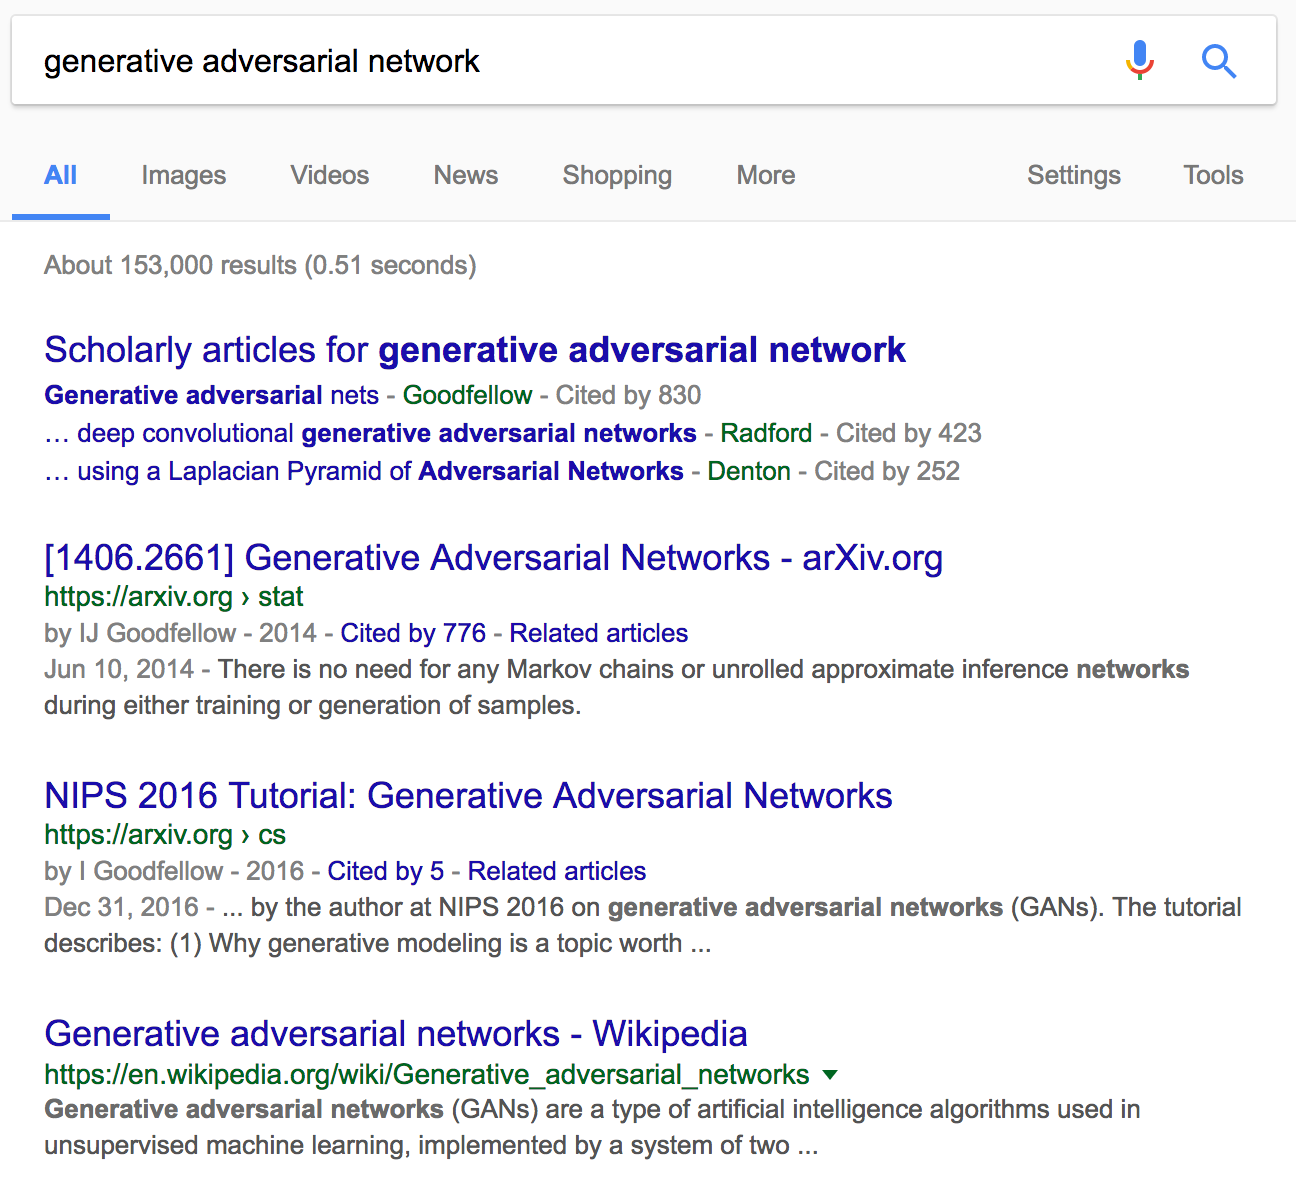
\includegraphics[height=0.6\textheight]{google_gan}
  \end{center}
  
  \begin{itemize}
  \item {
    Schmidhuber Review \url{https://media.nips.cc/nipsbooks/nipspapers/paper_files/nips27/reviews/1384.html}
  }
  \end{itemize}

\end{frame}

\begin{frame}{GANs}{}

  \begin{center}
    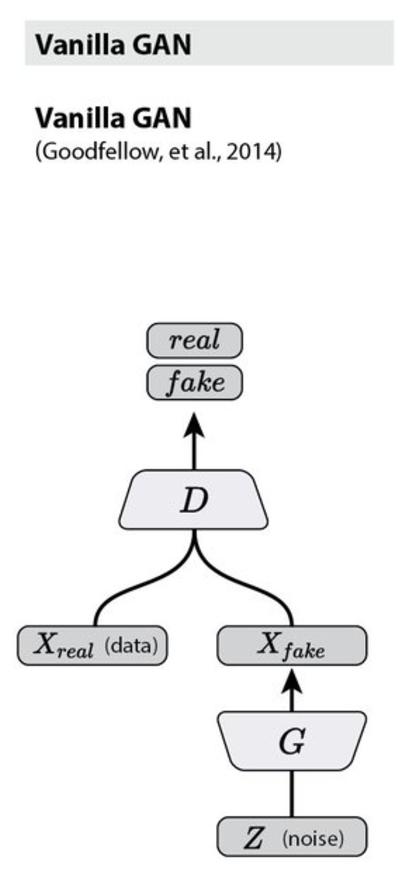
\includegraphics[height=0.6\textheight]{vanilla_gan}
  \end{center}
  
  \begin{itemize}
  \item {
    \url{https://twitter.com/ch402/status/793535193835417601}
  }
  \end{itemize}
\end{frame}

\begin{frame}[fragile]{GANs}{}

    Loss Function
    
    \begin{align*}
        \min_G \max_D V(D,G) = 
        \mathbb{E}_{x \sim p_{data}(x)} [ \log D(x) ] +
        \mathbb{E}_{z \sim p_z(z)} [ \log (1-D(G(z)) ]
    \end{align*}
  
\end{frame}

\begin{frame}[fragile]{GANs}{}

    Loss Function
    
    \begin{align*}
        \min_G \max_D V(D,G) = 
        \mathbb{E}_{x \sim p_{data}(x)} [ \log D(x) ] +
        \mathbb{E}_{z \sim p_z(z)} [ \log (1-D(G(z)) ]
    \end{align*}

\begin{center}
    \begin{lstlisting}[language=Python]
    real_x, fake_x = next_batch(), generator(z)
    z = sample_z()
    
    real_d = sigmoid(discriminator(real_x))
    fake_d = sigmoid(discriminator(fake_x))
    
    d_loss = - np.mean(np.log(real_d) + 
                       np.log(1. - fake_d))
    g_loss = - np.mean(np.log(fake_d))
    loss = d_loss + g_loss # or optimize separately
    \end{lstlisting}
\end{center}
  
\end{frame}

\begin{frame}{Visualizing GAN}{}

  \begin{center}
    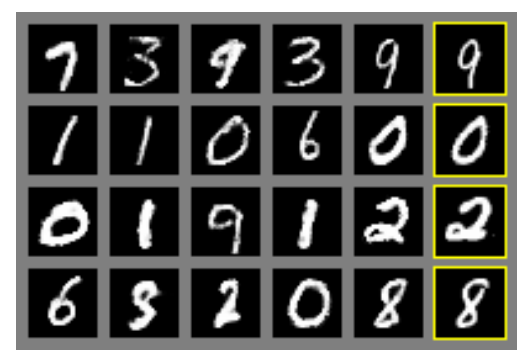
\includegraphics[height=0.6\textheight]{gan_neighbors}
  \end{center}
  
  From GAN paper.

\end{frame}

\begin{frame}{Visualizing GAN}{}

  \begin{center}
    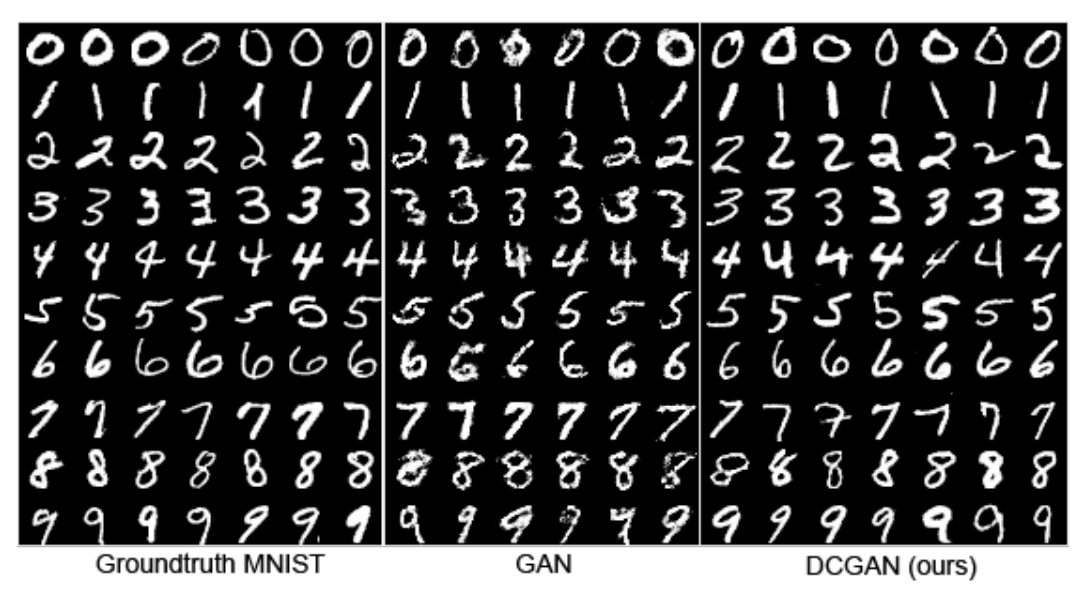
\includegraphics[height=0.6\textheight]{dcgan}
  \end{center}
  
  From DCGAN paper.

\end{frame}

\begin{frame}{Problem with Visualizing GANs}{}

  Can't specify the class.

\end{frame}

\begin{frame}{Information Maximization to the Rescue}{}

  We want to tie the class of the generated image to some input variable.

\end{frame}

\begin{frame}{Entropy}{}

  \begin{center}
    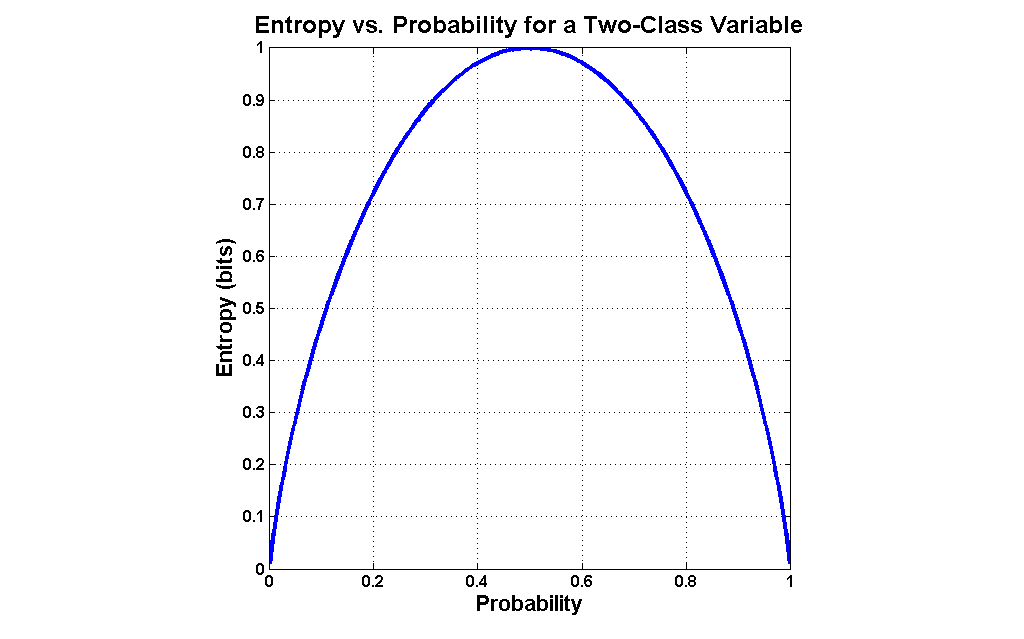
\includegraphics[height=0.6\textheight]{entropy}
  \end{center}

    \begin{align*}
        H(X) = - \frac{1}{N} \Sigma_x P(x) \log P(x)
    \end{align*}
    

\end{frame}

\begin{frame}{Conditional Entropy}{}
  
    \begin{align*}
        H(Y|X) 
        &= \Sigma_x P(x) H(Y|X=x) \\
        &= - \Sigma_x P(x) \Sigma_y P(y|x) \log P(y|x)
    \end{align*}

\end{frame}

\begin{frame}{Mutual Information}{}

  \begin{center}
    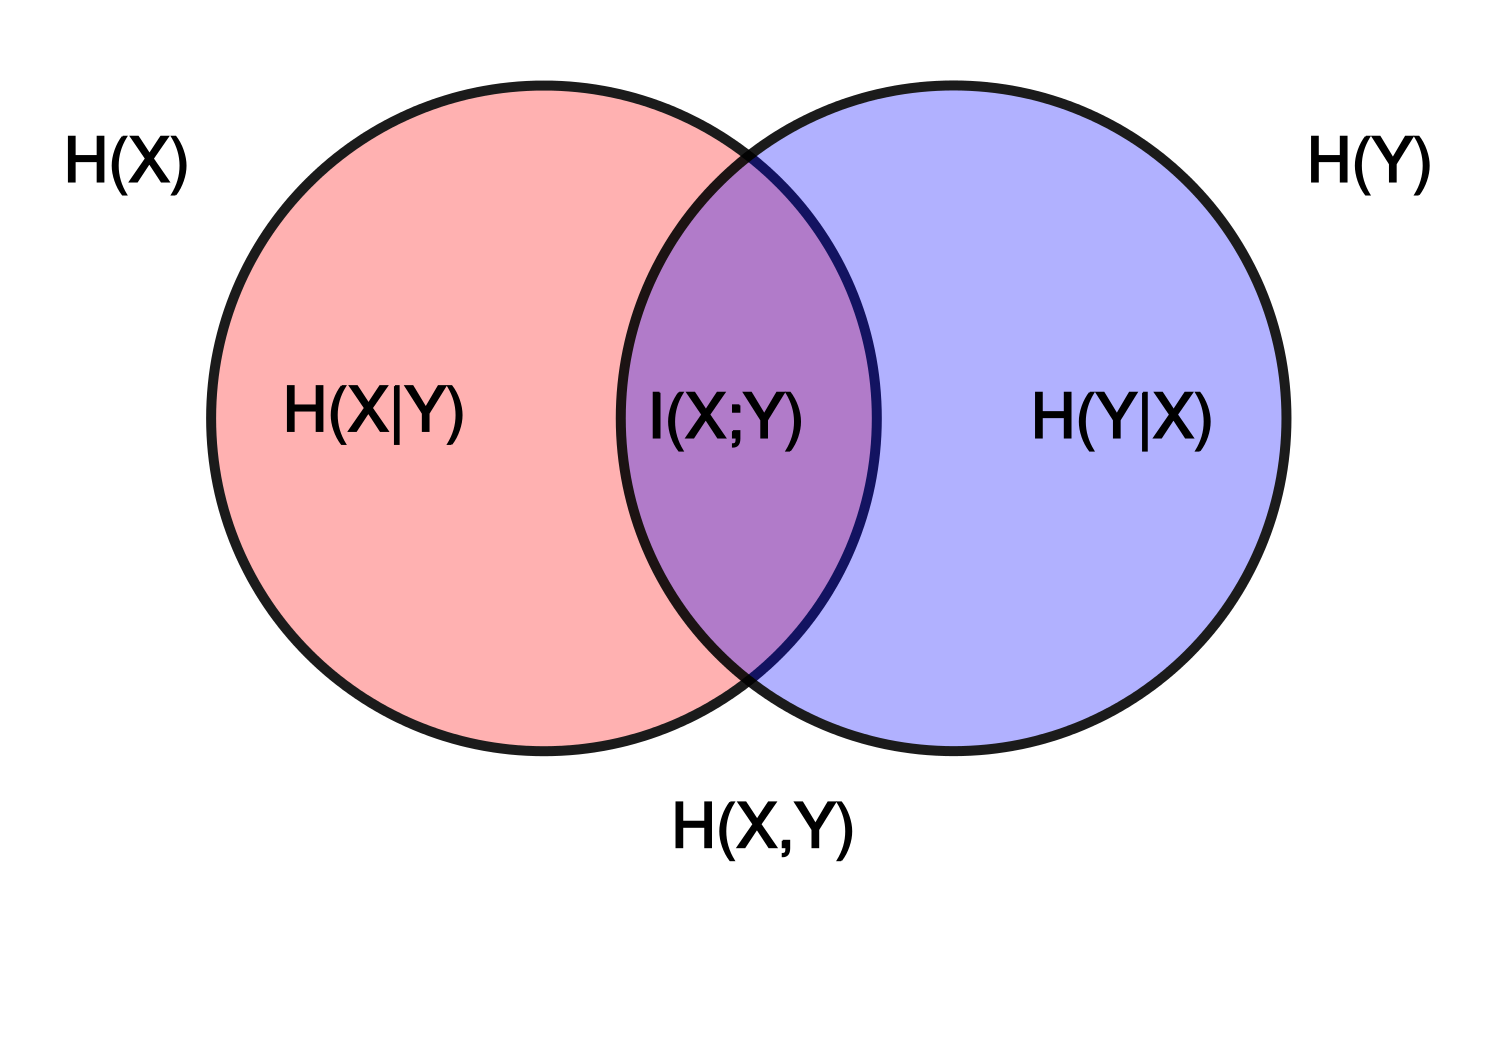
\includegraphics[height=0.5\textheight]{conditional_entropy}
  \end{center}
  
  \begin{align*}
        I(X;Y) &= H(X,Y)  \\
        &= H(X) - H(X|Y)  \\
        &= H(Y) - H(Y|X)
    \end{align*}

\end{frame}

\begin{frame}{KL Divergence}{}

  \begin{align*}
      D_{KL}(P||Q)
      &= \Sigma_x P(x) \log \frac{P(x)}{Q(x)} & \text{discrete} \\
      &= \int_{-\infty}^{\infty} P(x) \log \frac{P(x)}{Q(x)} & \text{continuous} \\
      &= \int_x P(x) \log \frac{P(x)}{Q(x)} & \text{general}
  \end{align*}
  
  \begin{itemize}
      \item It's always positive.
      \item It's asymmetric.
      \item It can serve as a distance metric between probability distributions.
  \end{itemize}

\end{frame}

\begin{frame}{InfoGAN}{}

\begin{center}
    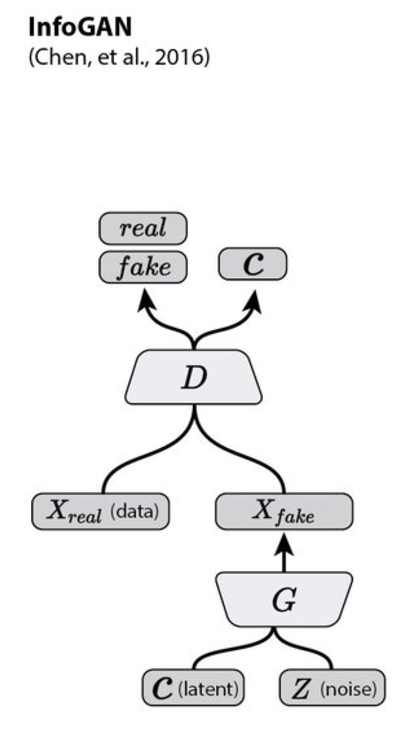
\includegraphics[height=0.6\textheight]{infogan}
\end{center}

\begin{itemize}
  \item {
    \url{https://twitter.com/ch402/status/793535193835417601}
  }
  \end{itemize}

\end{frame}

\begin{frame}{InfoGAN}{}

GAN Loss Function

\begin{center}
    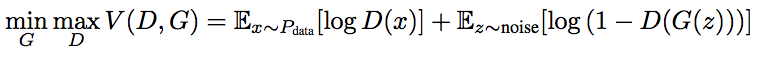
\includegraphics[width=0.8\textwidth]{gan_loss}
\end{center}

InfoGAN Loss Function

\begin{center}
    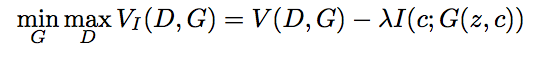
\includegraphics[width=0.55\textwidth]{infogan_loss}
\end{center}

\end{frame}

\begin{frame}{Derivation of the Lower Bound}{}

\begin{center}
    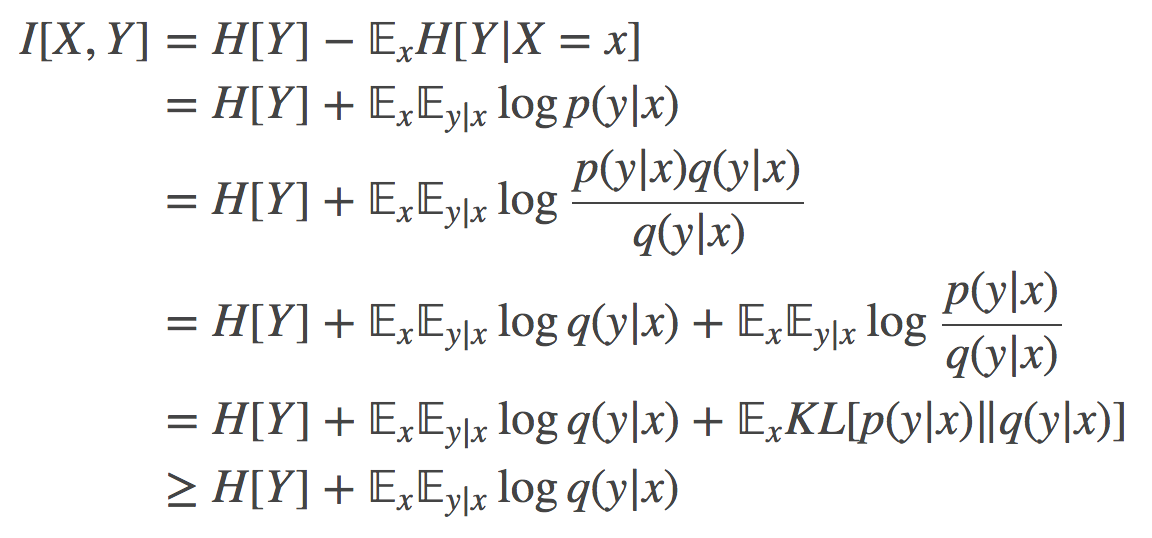
\includegraphics[height=0.6\textheight]{lowerbound}
\end{center}

  \url{http://www.inference.vc/infogan-variational-bound-on-mutual-information-twice/}

\end{frame}

\begin{frame}{Variational MI}{}

  This is the tricky part!

\end{frame}

\begin{frame}{Visualizing InfoGAN}{}

\begin{center}
    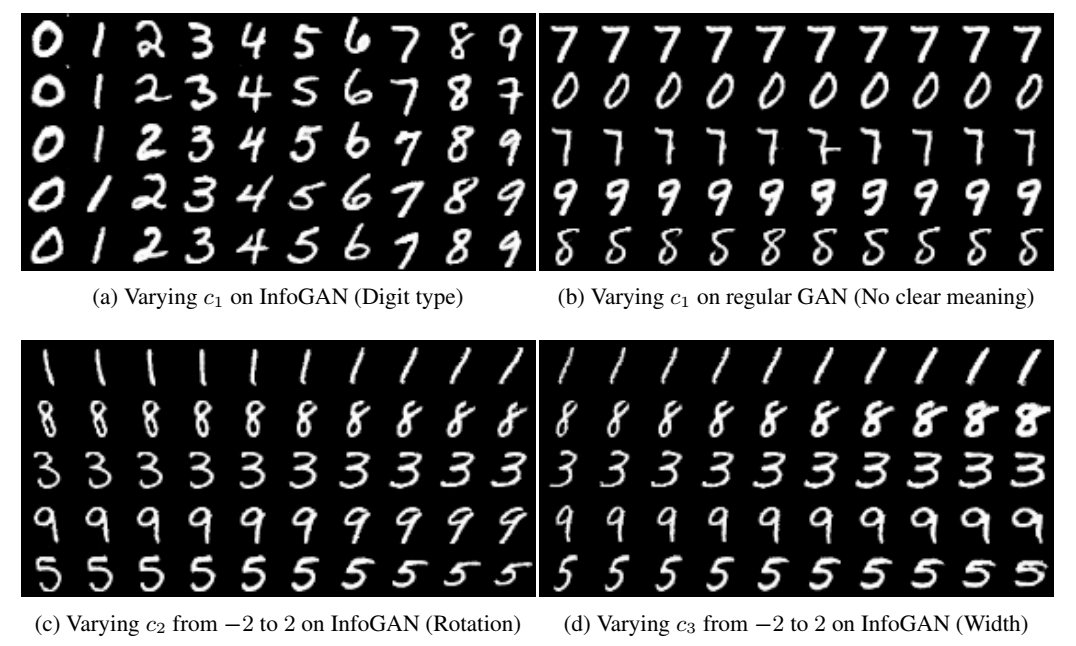
\includegraphics[height=0.6\textheight]{infogan_viz}
\end{center}

\end{frame}

\begin{frame}{Other Applications of Infomax and Mutual Information}{}

\begin{itemize}
  \item Stacked Denoising Autoencoders
  \item VIME
  \item Learning to Decode for Future Success
\end{itemize}

\end{frame}

\begin{frame}{Thanks!}{}

    \url{https://www.sharelatex.com/project/594ad735e0c50c8f165b7090}

\end{frame}


\end{document}


